% 保留原始面板、实拍、示例与全部连线；仅以 TikZ 覆盖说明标签。
\begin{tikzpicture}
\node[anchor=south west,inner sep=0] (im) at (0,0) {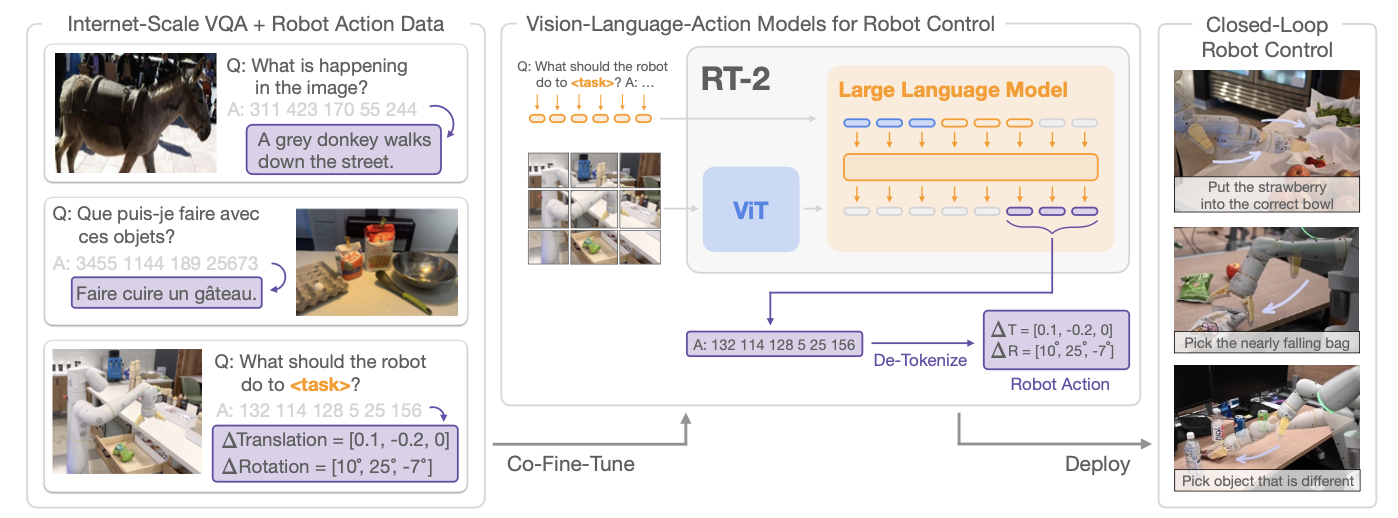
\includegraphics[width=\linewidth]{figures/rt2.png}};
\begin{scope}[x={(im.south east)},y={(im.north west)}]
\fill[white] (0.043634,0.930502) rectangle (0.317597,0.980695);
\node[align=center,inner sep=0pt,font=\fontsize{7.5}{8.5}\selectfont,text width=0.273963\linewidth,rotate=0] at (0.180615,0.955598) {互联网级 VQA 与机器人动作数据};
\fill[white] (0.371960,0.930502) rectangle (0.806152,0.978764);
\node[align=center,inner sep=0pt,font=\fontsize{8.5}{9.5}\selectfont,text width=0.434192\linewidth,rotate=0] at (0.589056,0.954633) {用于机器人控制的视觉语言动作模型};
\fill[white] (0.854077,0.874517) rectangle (0.968526,0.978764);
\node[align=center,inner sep=0pt,font=\fontsize{8.5}{9.5}\selectfont,text width=0.114449\linewidth,rotate=0] at (0.911302,0.926641) {闭环\\机器人控制};
\fill[orange!10] (0.596567,0.797297) rectangle (0.790415,0.849421);
\node[align=center,inner sep=0pt,font=\fontsize{9}{10}\selectfont,text width=0.193848\linewidth,rotate=0] at (0.693491,0.823359) {大语言模型};
\fill[white] (0.620172,0.281853) rectangle (0.697425,0.322394);
\node[align=center,inner sep=0pt,font=\fontsize{7.5}{8.5}\selectfont,text width=0.077253\linewidth,rotate=0] at (0.658798,0.302124) {反词元化};
\fill[white] (0.713162,0.223938) rectangle (0.800429,0.270270);
\node[align=center,inner sep=0pt,font=\fontsize{7.5}{8.5}\selectfont,text width=0.087268\linewidth,rotate=0] at (0.756795,0.247104) {机器人动作};
\fill[white] (0.360515,0.077220) rectangle (0.469957,0.129344);
\node[align=center,inner sep=0pt,font=\fontsize{8.5}{9.5}\selectfont,text width=0.109442\linewidth,rotate=0] at (0.415236,0.103282) {联合微调};
\fill[white] (0.756795,0.075290) rectangle (0.827611,0.135135);
\node[align=center,inner sep=0pt,font=\fontsize{8.5}{9.5}\selectfont,text width=0.070815\linewidth,rotate=0] at (0.792203,0.105212) {部署};
\fill[gray!15] (0.842632,0.590734) rectangle (0.972818,0.658301);
\node[align=center,inner sep=0pt,font=\fontsize{6.5}{7.5}\selectfont,text width=0.130186\linewidth,rotate=0] at (0.907725,0.624517) {草莓放入正确的碗中};
\fill[gray!15] (0.842632,0.050193) rectangle (0.973534,0.100386);
\node[align=center,inner sep=0pt,font=\fontsize{6.5}{7.5}\selectfont,text width=0.130901\linewidth,rotate=0] at (0.908083,0.075290) {挑出不同的物体};
% 完整中文化问答示例；数值词元、占位符、照片与连线保持原样。
\fill[white] (0.158798,0.808880) rectangle (0.317597,0.895753);
\node[anchor=north west,align=left,inner sep=0pt,font=\fontsize{6.2}{7.1}\selectfont,text width=0.155937\linewidth] at (0.160229,0.891892) {问：图像中发生了什么？};
\fill[violet!14] (0.178112,0.669884) rectangle (0.313305,0.752896);
\node[anchor=center,align=center,inner sep=0pt,font=\fontsize{6.2}{7.1}\selectfont,text width=0.132332\linewidth] at (0.245708,0.711390) {一头灰驴走在街上。};
\fill[white] (0.035765,0.517375) rectangle (0.209585,0.604247);
\node[anchor=north west,align=left,inner sep=0pt,font=\fontsize{6.2}{7.1}\selectfont,text width=0.170959\linewidth] at (0.037196,0.600386) {问：这些东西能做什么？};
\fill[violet!14] (0.053648,0.415058) rectangle (0.185980,0.459459);
\node[anchor=center,align=center,inner sep=0pt,font=\fontsize{6.2}{7.1}\selectfont,text width=0.129471\linewidth] at (0.119814,0.437259) {烤一个蛋糕。};
\fill[white] (0.153076,0.229730) rectangle (0.319742,0.322394);
\node[anchor=north west,align=left,inner sep=0pt,font=\fontsize{6.2}{7.1}\selectfont,text width=0.163805\linewidth] at (0.154506,0.318533) {问：机器人如何完成\texttt{<task>}？};
\fill[violet!14] (0.154506,0.077220) rectangle (0.324034,0.171815);
\node[anchor=center,align=center,inner sep=0pt,font=\fontsize{6.0}{7.2}\selectfont,text width=0.166667\linewidth] at (0.239270,0.124517) {$\Delta\text{平移}=[0.1,-0.2,0]$\\$\Delta\text{旋转}=[10^\circ,25^\circ,-7^\circ]$};
\fill[white] (0.367668,0.820463) rectangle (0.479971,0.895753);
\node[anchor=north west,align=left,inner sep=0pt,font=\fontsize{4.8}{5.4}\selectfont,text width=0.109442\linewidth] at (0.369099,0.891892) {问：机器人如何\\完成\texttt{<task>}？答：…};
\fill[gray!15] (0.840486,0.590734) rectangle (0.975680,0.656371);
\node[anchor=center,align=center,inner sep=0pt,font=\fontsize{6.0}{6.8}\selectfont,text width=0.132332\linewidth] at (0.908083,0.623552) {把草莓放入正确的碗中};
\fill[gray!15] (0.841917,0.322394) rectangle (0.970672,0.357143);
\node[anchor=center,align=center,inner sep=0pt,font=\fontsize{6.0}{6.8}\selectfont,text width=0.125894\linewidth] at (0.906295,0.339768) {拿起即将掉落的袋子};
\end{scope}
\end{tikzpicture}
